\subsection{The \kpimm invariant mass distribution}
\label{sec:kpimm:massfit}

The $m(\Kp\pim\mumu)$ invariant mass is used to discriminate between signal and background. The signal distribution is modelled using the sum of two Gaussian functions with a common mean, each with a power-law tail on the low-mass side.  The combinatorial background is modelled using an exponential function.  The parameters describing the shape of the mass distribution of the signal are determined from a fit to the \BdToJPsiKstP decay in the data, as shown in Fig.~\ref{fig:massfit}, and are subsequently fixed when fitting the \BdToKpimm candidates. A single scaling factor is used to correct the width of the Gaussian functions to account for variations in the shape of the mass distribution of the signal observed in simulation, due to the different regions of \mkpi and \qsq between the control mode and signal mode.  An additional component is included to model the contribution from \BsToJPsiKst in the fit to the control mode. % which is neglected when fitting the \BdToKpimm candidates.
The fit to \BdToKpimm candidates in the range $1.1 < \qsq < 6.0\gevgevcccc$ is shown in Fig.~\ref{fig:massfit}. The signal yield in the range $1.1 < \qsq < 6.0\gevgevcccc$ is $229 \pm 21$.
 
\begin{figure}[!tb]
\centering
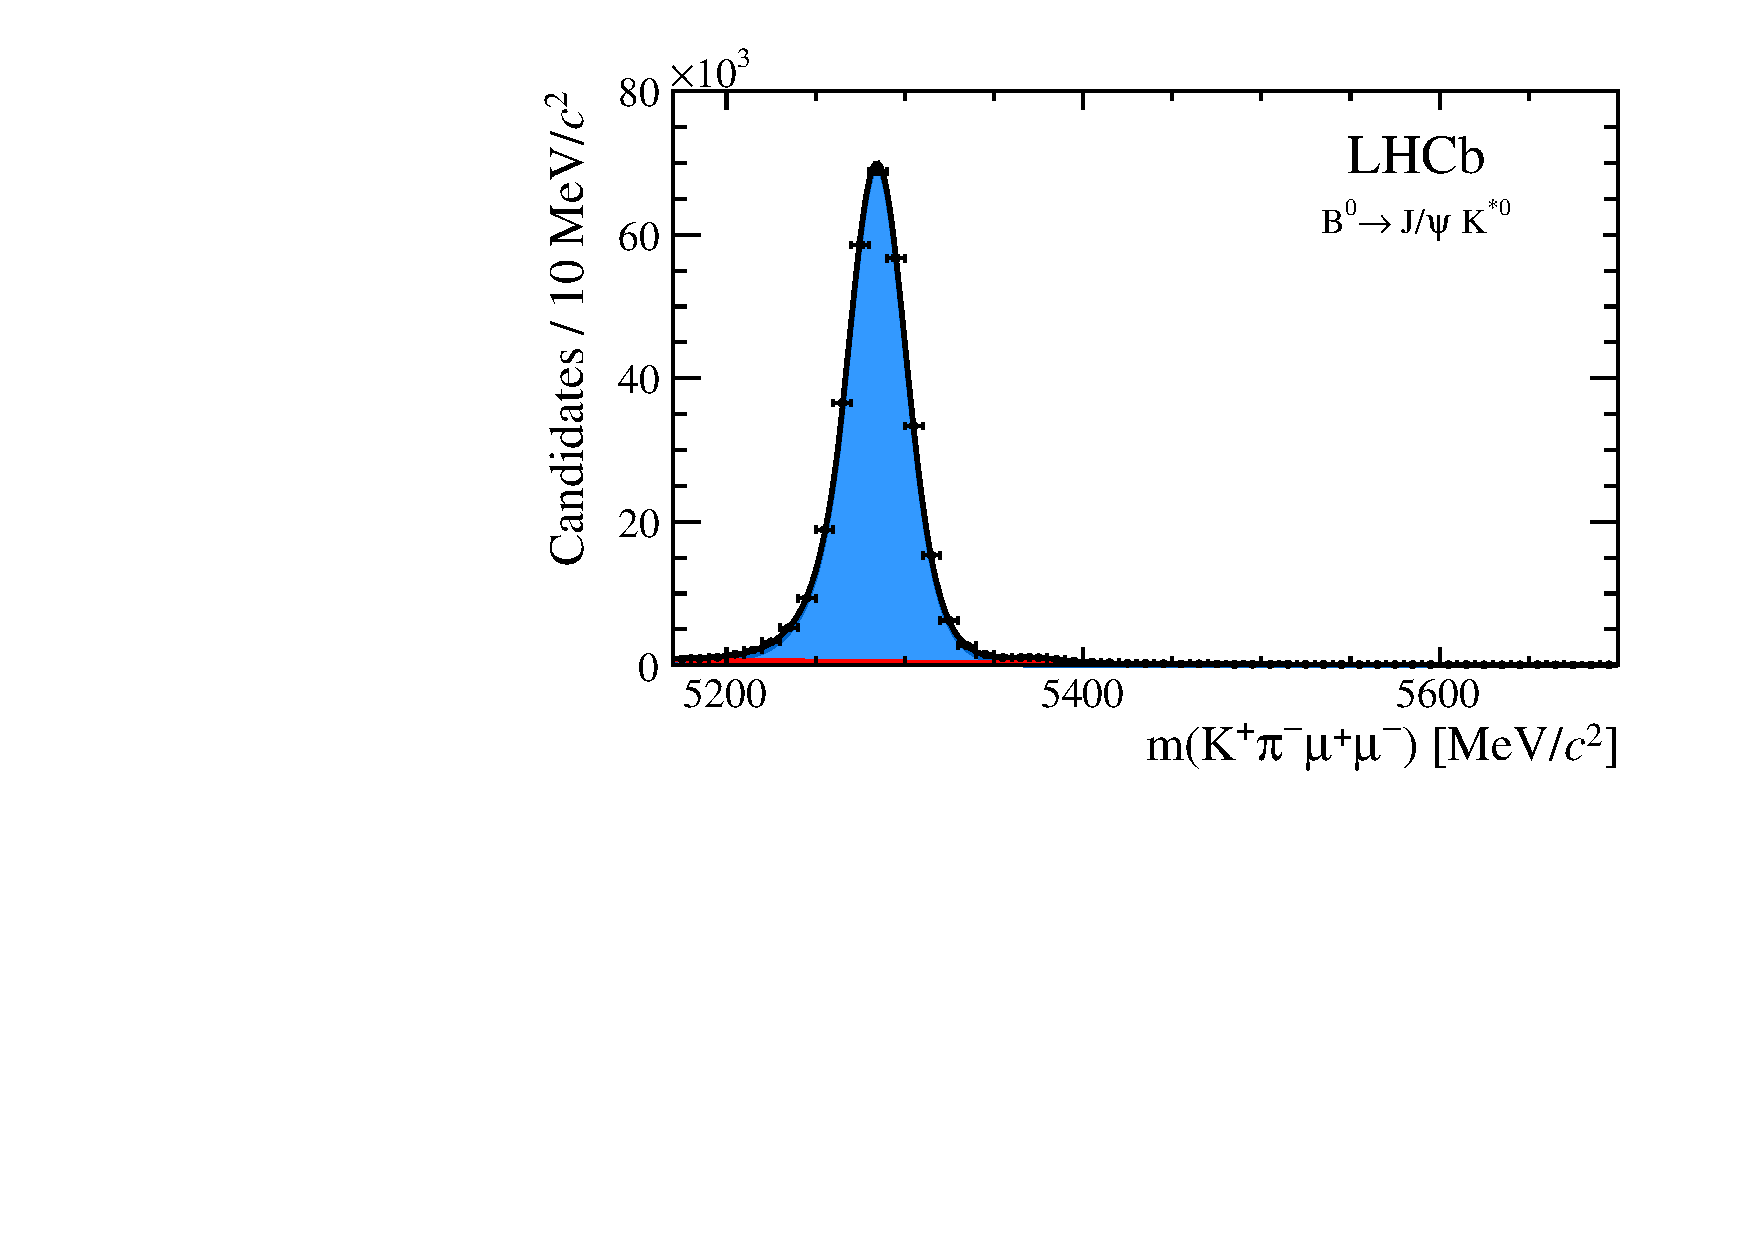
\includegraphics[width=0.48\linewidth]{figs/kpimm/massfit/fit_jpsi.pdf}
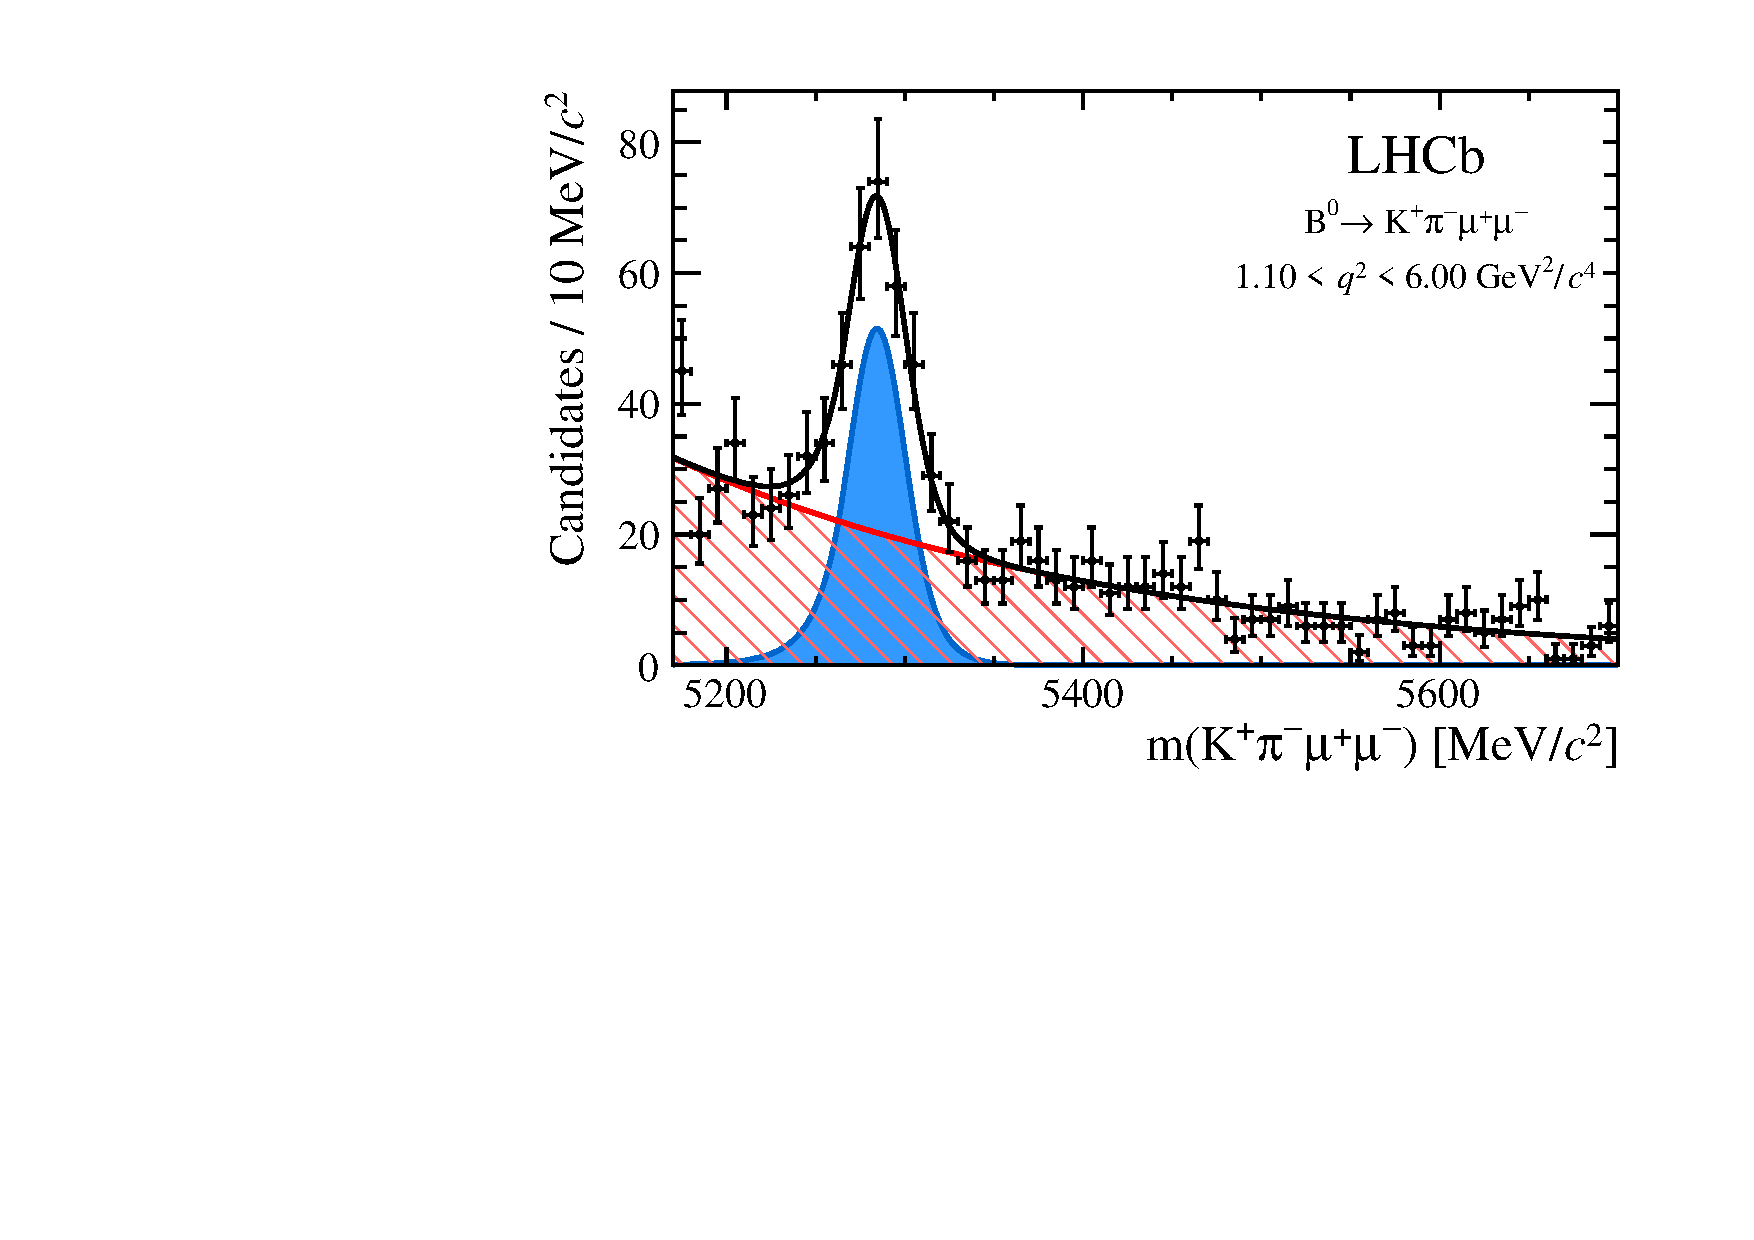
\includegraphics[width=0.48\linewidth]{figs/kpimm/massfit/fitKpimumu_q2_1p1_6p0.pdf}
\caption{Invariant mass \mkpimm for (left) the control decay \BdToJPsiKst and (right) the signal decay \BdToKpimm in the bin $1.1 < \qsq < 6.0\gevgevcccc$. The solid black line represents the total fitted function.  The individual components of the signal (blue shaded area) and combinatorial background (red hatched area) are also shown.}
\label{fig:massfit}
\end{figure}